\section{Proposed HRDNUT Latch Design} \label{Proposed}
In this section we discuss the proposed DNU robust latch. The latch implementation is based on three cross connected storage loops connected to three C-elements. The basic design of the storage loop is given in Fig. \ref{Block}. The data loop is based on the standard latch design with a 3-input C-element inserted to replace one of the inverters. The purpose of the C-element is to separate the feedback loop so that an error will not be held. Additionally, a PMOS is connected to the positive clock signal (CLK) and a NMOS is connected to the negative clock signal (CLKB) to remove contention when data is loaded to the latch. As in the modified DONUT latch, the addition of these transistors drastically reduces the delay and power consumption.    

\begin{figure}[h]
	\centering
	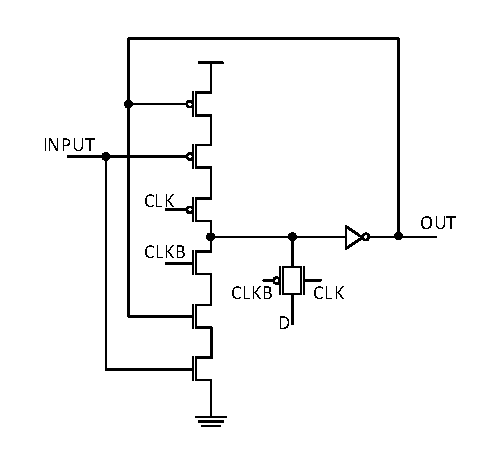
\includegraphics[width=0.5\linewidth]{Figures/Block}
	%where an .eps filename suffix will be assumed under latex, 
	%and a .pdf suffix will be assumed for pdflatex; or what has been declared
	%via \DeclareGraphicsExtensions.
	\caption{Basic data storage loop block.}
	\label{Block}
\end{figure} 

Using the basic storage block we construct the block based latch as in Fig. \ref{BLatch}. The latch was designed with the goal of ensuring that none of the nodes directly drove itself. For example, it can see that in Fig. \ref{Block} the node \textit{out} is fed into the input of the 3-input C-element. If an error strikes node \textit{out}, the cell will never be able to recover its previous state since one of the C-element inputs will be held to an erroneous value by its output. To prevent this issue, our design is based on cross-connecting three of the storage loop blocks so that the C-element is driven by three separate block outputs. In Fig. \ref{BLatch} we provide a basic latch design using this idea. If a single error occurs on any node in this design, the circuit is capable fully recovering the previous data. 

To demonstrate this, consider a strike on node \textit{n2}. When the strike occurs, the erroneous value will be propagated to the C-elements driving nodes \textit{n1} and \textit{n3}. However, since there is no change on \textit{n1} or \textit{n3}, the C-elements \textit{C1} and \textit{C3} will hold their previous value thus preventing the error from propagating to the output. Additionally, since node \textit{n2} is driven by nodes \textit{n1} and \textit{n3}, \textit{n2} will completely recover the correct state. 

\begin{figure}[!htbp]
	\centering
	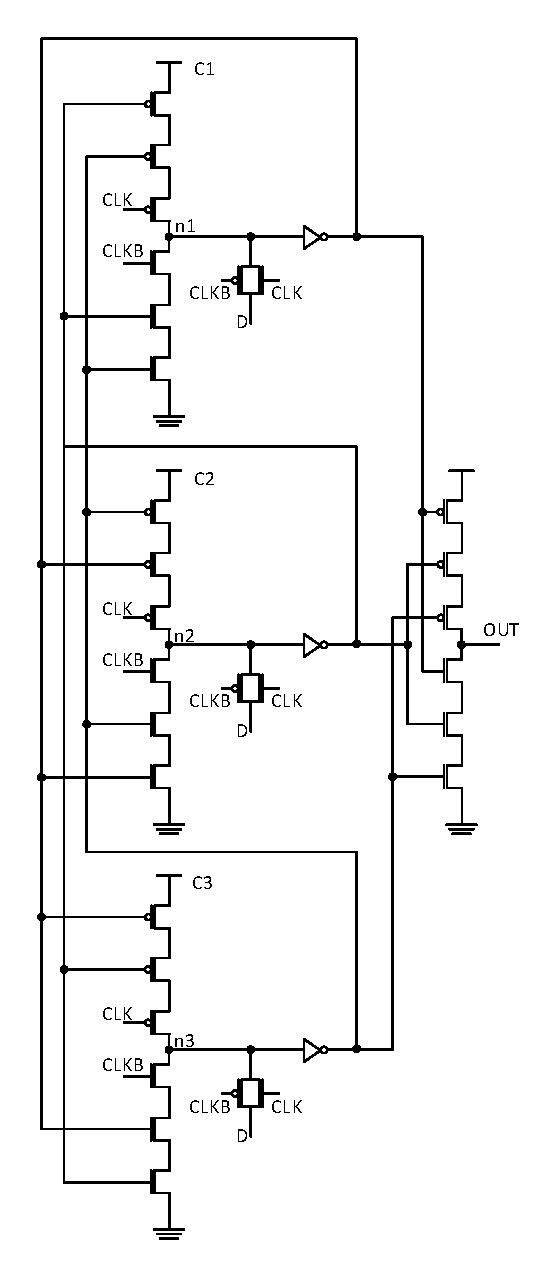
\includegraphics[width=0.55\linewidth]{Figures/BLatch}
	%where an .eps filename suffix will be assumed under latex, 
	%and a .pdf suffix will be assumed for pdflatex; or what has been declared
	%via \DeclareGraphicsExtensions.
	\caption{Schematic of the block-based latch.}
	\label{BLatch}
\end{figure} 

A problem, however, with the latch in Fig. \ref{BLatch} is that it is not capable of tolerating DNUs. For example, if an error occurs on nodes \textit{n1} and \textit{n2} the erroneous values will propagate to the inputs of C-element \textit{C3} and flip the value of \textit{n3} thus changing the output value. However, since the latch has recovery capability for SEUs, we modify it so it can tolerate DNUs and recover all nodes to the previous state. In Fig. \ref{HRDNUT} we provide the schematic of the proposed HRDNUT latch. The design uses the block-based latch in Fig. \ref{BLatch} as a base and adds additional C-elements to prevent errors from being held by the data loop.  

Initially, we will evaluate the HRDNUT latch during normal operation. When the positive clock signal (CLK) has a high value and the negative clock signal (CLKB) has a low value, the latch is in transparent mode. At this stage, the transistors connected to the clock signal in C-element \textit{C1} deactivates the PMOS and NMOS stacks thus causing the node \textit{n1} to be in a high impedance state. This, in effect, reduces data contention thus reducing delay and dynamic power consumption. Next, the data is loaded through the pass gates connected to nodes \textit{n1}, \textit{n22} and \textit{out}. Since the output node \textit{out} is loaded directly, the data to out delay is minimized and all nodes are set to their respective error free values. When CLK changes to a low value and CLKB to a high value, the latch moves into the hold mode. In this stage, the pass gates are deactivated and the state of the latch is held since each node is driven to the correct value using a C-element. Fig. \ref{NormOp} provides the waveforms of the CLK, D and OUT nodes for both the transparent and hold modes of operation.

\begin{figure}[!htbp]
	\centering
	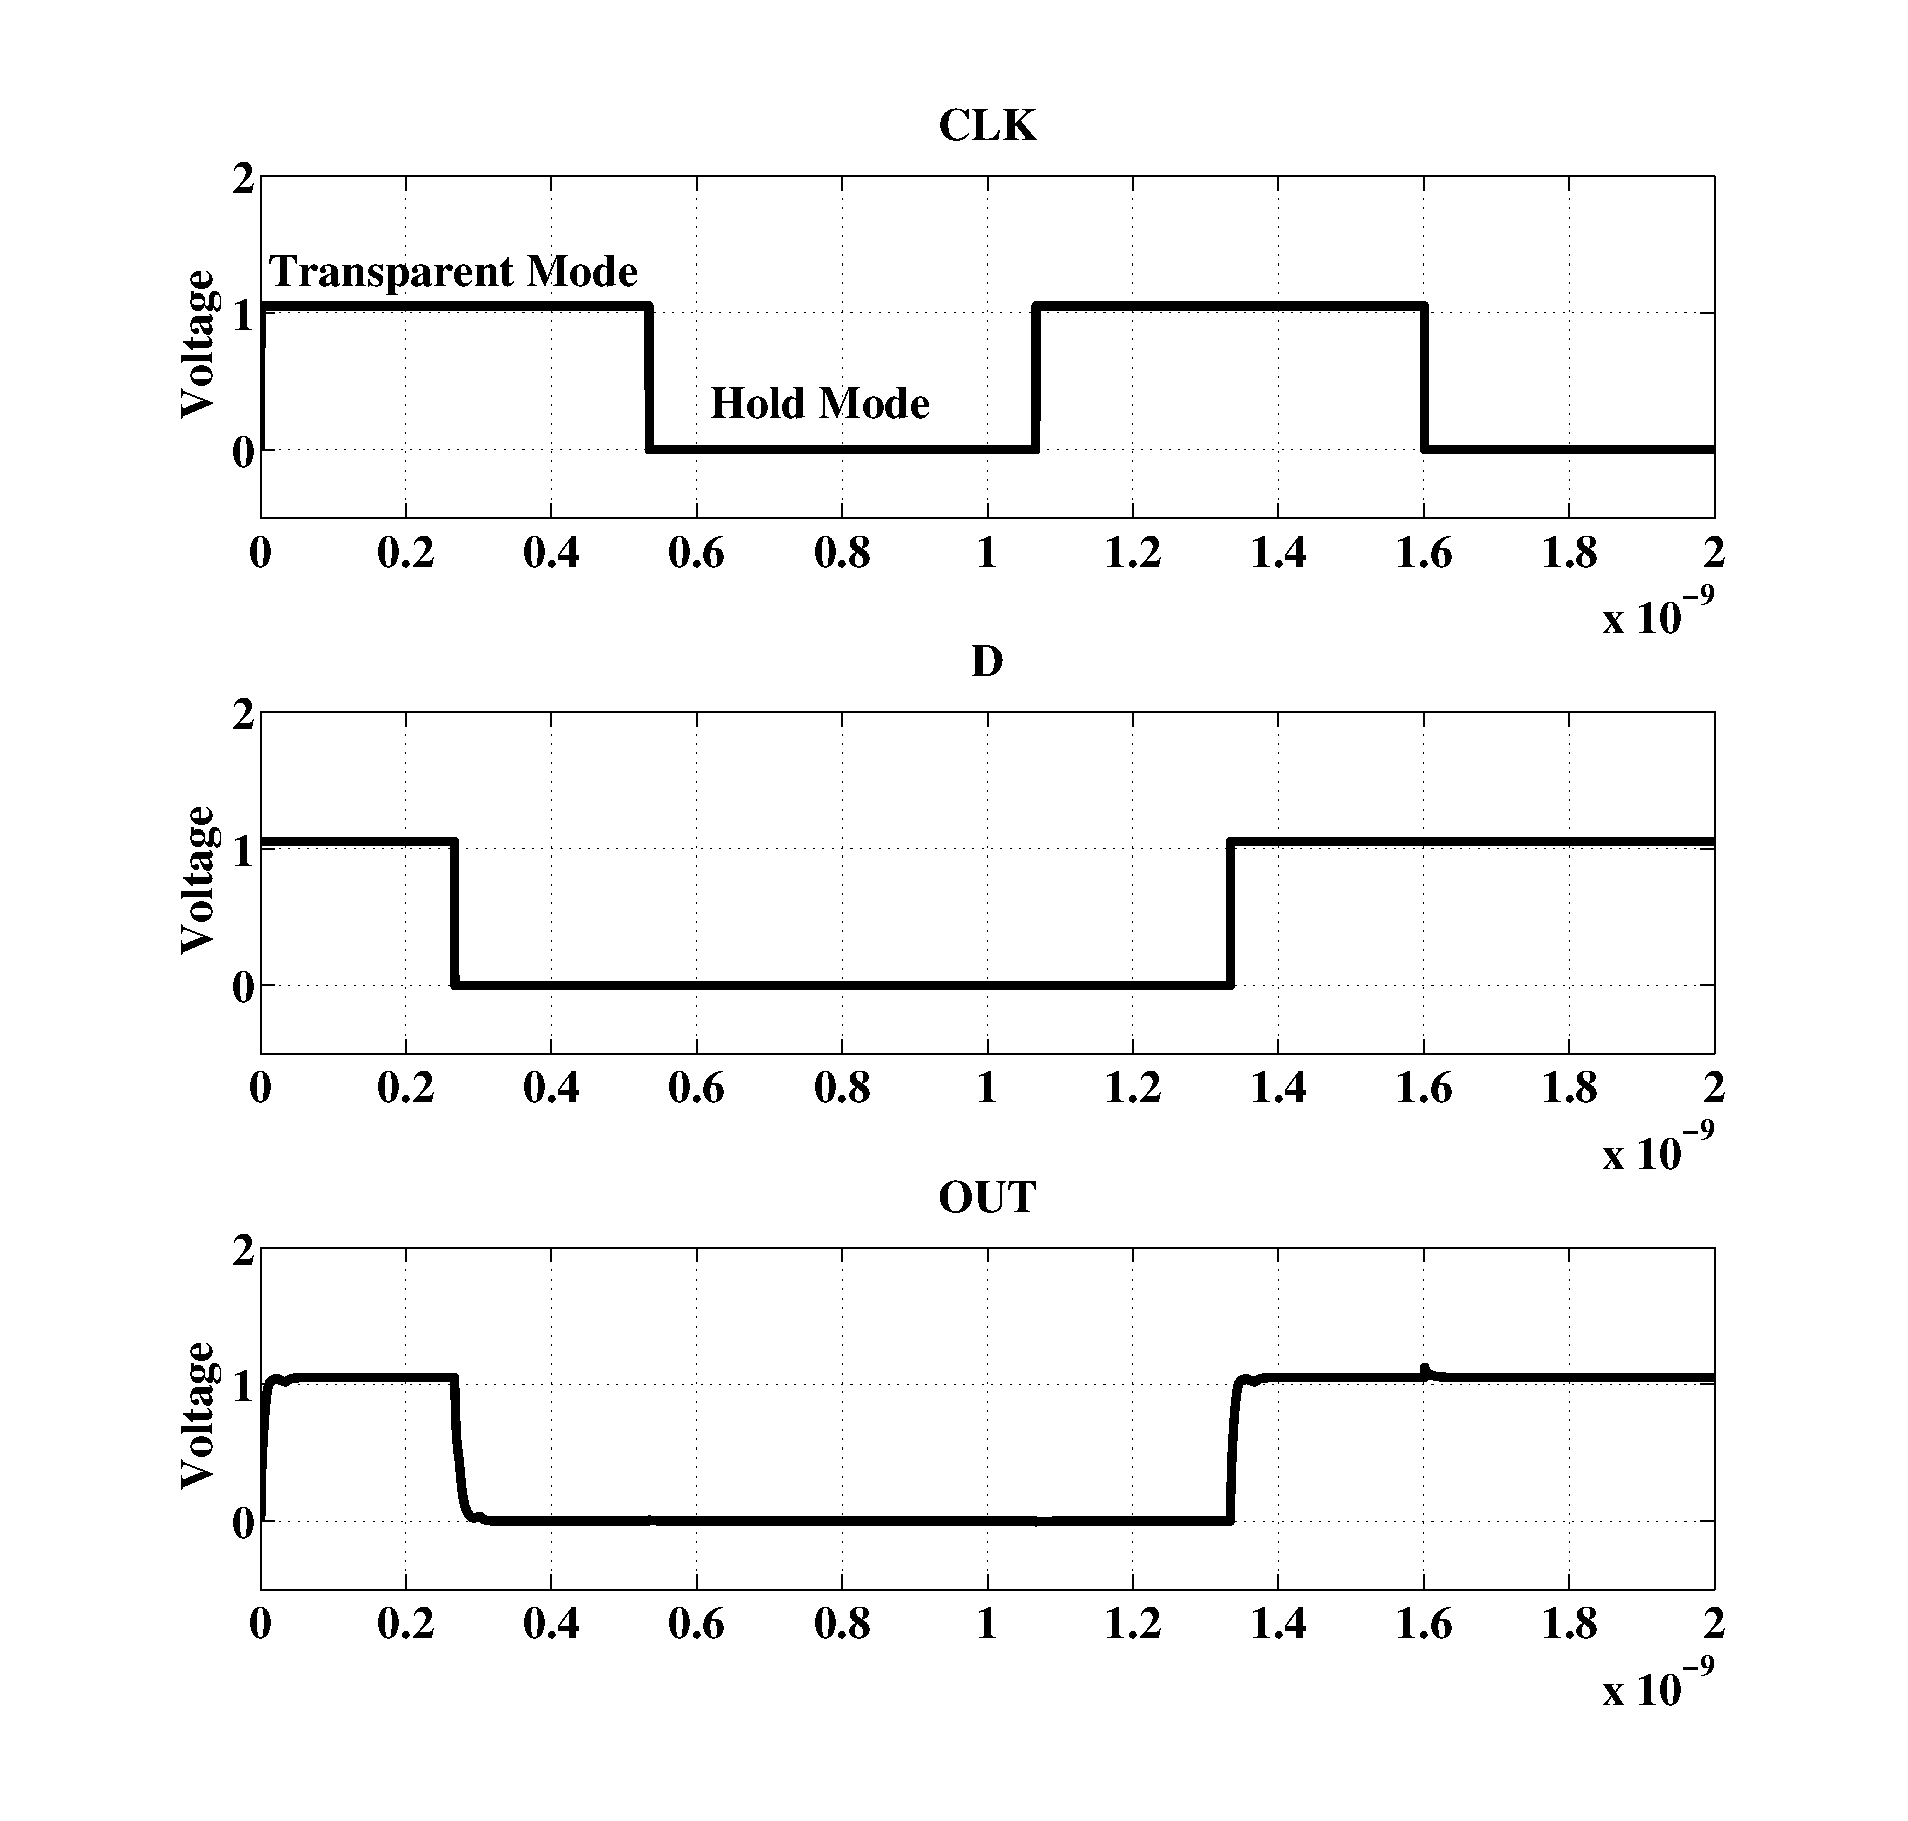
\includegraphics[width=0.80\linewidth]{Figures/defaultoperation.eps}
	%where an .eps filename suffix will be assumed under latex, 
	%and a .pdf suffix will be assumed for pdflatex; or what has been declared
	%via \DeclareGraphicsExtensions.
	\caption{Waveforms of the HRDNUT latch during normal operation.}
	\label{NormOp}
\end{figure}

In the case of an SEU, the HRDNUT retains the excellent resiliency of the block based latch and the ability to recover every node after an error. In the case of any internal node being struck by an error, the latch will not change value due to all internal C-elements requiring at least 2 identical input values to change values. In the case of an error hitting the output node \textit{out}, the latch fully recovers since \textit{out} does not directly drive C-element \textit{C7}.

\begin{figure}[!tbp]
	\centering
	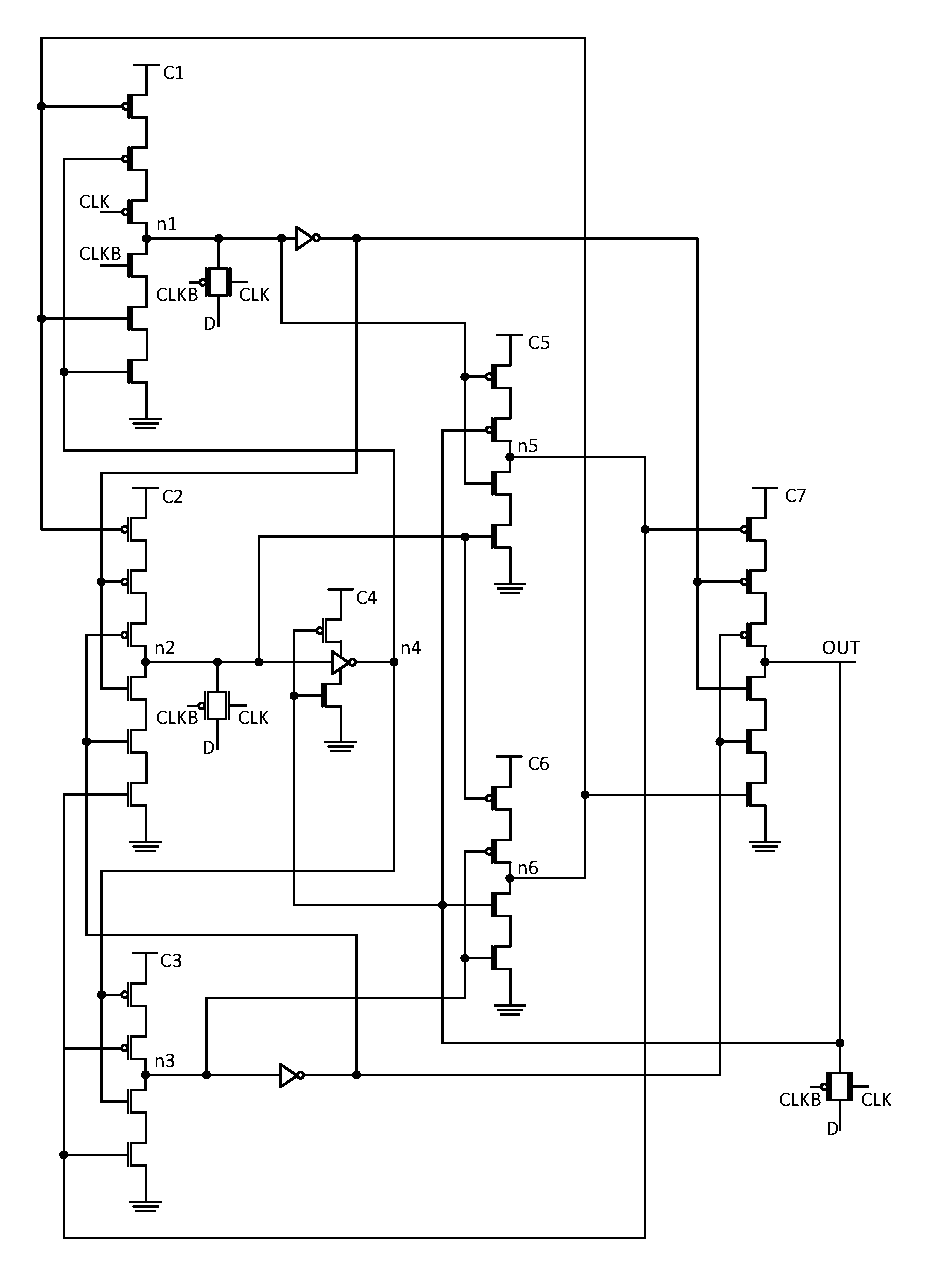
\includegraphics[width=\linewidth]{Figures/HRDNUT}
	%where an .eps filename suffix will be assumed under latex, 
	%and a .pdf suffix will be assumed for pdflatex; or what has been declared
	%via \DeclareGraphicsExtensions.
	\caption{Schematic of the HRDNUT latch.}
	\label{HRDNUT}
\end{figure} 

Lastly, we will evaluate the latch in the case of a DNU. Note that unless otherwise stated, it is assumed that the analysis applies to both when D=0 and D=1. For our analysis, we categorize the possible DNU strike combinations into 9 distinct cases based on their effect in the HRDNUT latch. The categories are discussed in detail below:

\begin{enumerate}
	\item Consider strikes at nodes \textit{n1} and \textit{n2}. In this case, the error at \textit{n1} will propagate to C-elements \textit{C5} and \textit{C7} but will not cause a flip since the error at \textit{n2} will be blocked by C-element \textit{C4}. Additionally, since the inputs of C-elements \textit{C1} and \textit{C2} are unchanged, the nodes will recover their initial values. This analysis can be applied to node combinations containing node \textit{n2} except for the combination with node \textit{out} since the error will be blocked by C-element \textit{C4}.
	
	\item In the case of a DNU upsetting nodes \textit{n2} and \textit{out}, the error at \textit{n2} will propagate through C-element \textit{C4}. However, C-elements \textit{C1} and \textit{C3} will block the error and nodes \textit{n1}, \textit{n3}, \textit{n5} and \textit{n6} will hold their values thus driving node \textit{out} to the correct state. 

	\item Consider when a DNU strikes nodes \textit{n1} and \textit{n5}. In this case, the error at \textit{n1} hits the output of C-element \textit{C1} which is propagated to \textit{C7}. The error on \textit{n5} is also propagated to C-element \textit{C7}. Since node \textit{n3} and the inputs of C-elements \textit{C1} and \textit{C5} are unaffected by an error, the output retains the error-free value and the latch fully recovers the previous state. The above analysis also applies to the node combination (\textit{n3}, \textit{n6}).

	\item In the case of a DNU hitting nodes \textit{n3} and \textit{n4}, the error at \textit{n4} is propagated to C-element \textit{C3} and the error at \textit{n3} is propagated to \textit{C7} and \textit{C6}. After the error on \textit{n3} subsides, \textit{C4} will drive node \textit{n4} and, due to the connection at \textit{C3}, node \textit{n3} back to the error-free value. The node combination (\textit{n1}, \textit{n1}) can be analyzed similarly. For the node combinations of (\textit{n4}, \textit{n5}) and (\textit{n4}, \textit{n6}), the latch will also recover the previous result since the inputs to \textit{C4} are unchanged. This implies that after the error occurs at \textit{n4}, the node will be driven back to the correct value thus also driving the nodes \textit{n5} or \textit{n6} back to the correct value.
	
	\item When a DNU upsets the combination of \textit{n4} and \textit{out}, the error at \textit{out} is propagated to \textit{C4}, \textit{C5} and \textit{C6} and the error at \textit{n4} to \textit{C1} and \textit{C3}. Since none of the inputs to \textit{C7} are changed by the error, \textit{out} is flipped back to its error-free value which drives \textit{n4} through \textit{C4} back to its previous state.

	\item Consider when a DNU strikes nodes \textit{n1} and \textit{n3} being struck. In this case, the errors are propagated to C-elements \textit{C2}, \textit{C5}, \textit{C6} and \textit{C7}. However, since the errors do not manifest into an error on any other node, the latch fully recovers from the error. 
	
	\item When a DNU strikes the nodes \textit{n1} and \textit{n6}. The error at node \textit{n6} propagates to  \textit{C1} and \textit{C7} while the error at \textit{n1} also propagates to \textit{C7}. Due to the error-free node \textit{n3} driving \textit{C7}, the previous value is held at the output by \textit{C7}. Additionally, \textit{n3} will drive \textit{C6} back to its previous value thus driving \textit{C1} back to the error free state. This analysis can be applied similarly to the node combination of (\textit{n3}, \textit{n5}). 

	\item In the case where a DNU strikes nodes \textit{n5} and \textit{out} the error at \textit{n5} propagates to \textit{C7}, \textit{C2} and \textit{C3} and the error at \textit{out} goes to \textit{C4}, a PMOS in \textit{C5} and a NMOS in \textit{C6}. When the error-free value at \textit{out} is 1, the value at \textit{n5} is 0. The error at the nodes change the values to 0 and 1 respectively and the erroneous value at \textit{out} is propagated to the PMOS at \textit{C5} and the NMOS at \textit{C6}. This, in effect, causes the PMOS at \textit{C5} to be activated and the NMOS at \textit{C6} to be deactivated. However, since nodes \textit{n1} and \textit{n2} remain error-free, the NMOS stack of \textit{C5} will drive \textit{n5} back to the correct value. This, in turn, forces \textit{C7} to also drive \textit{out} back to the error-free value. In the case where \textit{out} has an ideal value of 0, the error will be fully recovered since the NMOS stack will be entirely driven by fault-free nodes. The above analysis can be applied to the node combination of (\textit{n6}, \textit{out}). 
	
	\item Lastly, we analyze the node combinations (\textit{n1}, \textit{out}), (\textit{n3}, \textit{out}) and (\textit{n5}, \textit{n6}). In these cases the errors do not cause a change on the inputs of any C-elements driving the node thus the previous value will always be recovered. 
\end{enumerate}